\section{Attitude Estimation}
In this part of our project, we tend to obtain accurate attitude estimates that will help us in computing a suitable control action. In our system we have Gyro and magnetometer sensors that provide us with measurements of angular rates, magnetic field, and acceleration components. To have accurate estimates to the actual internal states, we use Extended Kalman Filter (EKF) to combine the system model with the measurements. For the altitude to be estimated we need to define and implement a State observer. State observer is the mathematical model that represents the real system and gives the internal state estimates depending on input and output signals.  
\begin{align}
    \mathbf{\hat{x}}_k &= f(\mathbf{x}_k, \mathbf{u}_k) + \mathbf{w}_k \\
    \mathbf{\hat{z}}_k &= h(\mathbf{x}_k) + \boldsymbol{\nu}_k
\end{align}
where: \\
$\mathbf{\hat{x}}_k$: is the internal state vector.\\
$\mathbf{u}_k$:  is input signals at time k.\\
$f(\mathbf{x}_k, \mathbf{u}_k)$: is the function that relates the states at time $k + 1$ to the previous state $\mathbf{\hat{x}}_k$ and input $\mathbf{u}_k)$. \\
$\mathbf{\hat{z}}_k$: is the system output.\\
$ h(\mathbf{x}_k)$: relates the internal states to the output.\\
$\mathbf{w}_k$, $\boldsymbol{\nu}_k$: are the noises which are both assumed to be zero mean multivariate Gaussian noises with covariance $\mathbf{P}_k$ and $\mathbf{Q}_k$ respectively. 
The block diagram for the problem is defined in \ref{fig:est}.

\begin{figure}[H]
    \centering
    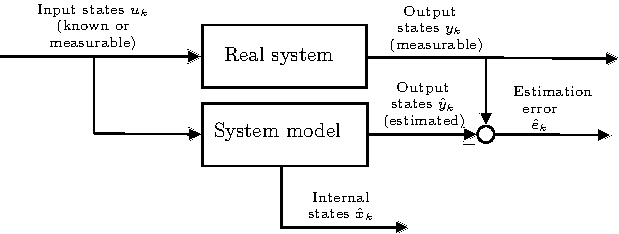
\includegraphics{Figures/estimation.pdf}
    \caption{block diagram for the estimation problem formulation}
    \label{fig:est}
\end{figure}
The estimation error $\mathbf{e}_k$ is the difference between the real system output and the estimated output. A very common way to minimize the variance of this estimation error is the Kalman Filters. The standard Kalman filter is a recursive filter that works in two steps:
\begin{enumerate}
    \item predicting the altitude based on the mathematical models.
    \item updating this altitude based on the data we get from sensors.
\end{enumerate}
For each new data from the sensor, is complained with the estimated state of the previous time step $\mathbf{x}_{k-1}$ to have a new update for the altitude $\mathbf{x}$ (state estimate) and the error covariance matrix (the accuracy of the estimate $\mathbf{P}$) this is called the time update step. The second step is the state correction. It mainly depends on the state vector covariance matrix $\mathbf{P}_{k}$.
\begin{align}
    \mathbf{\hat{x}}_{0}^{+} &= \mathbb{E}(\mathbf{x}_0)\\
    \mathbf{P}_{0}^{+} &= \mathbb{E} \left \{(\mathbf{x}_0 - \mathbf{\hat{x}}_0^{+}) (\mathbf{x}_0 - \mathbf{\hat{x}}_0^{+})^{\text{T}} \right \}
\end{align}
KF works as a least square error optimizer, this means that the system we have must be a linear system \cite{hasan2006review}.For a discrete-time nonlinear dynamic system -like ours- we use a modified version of the KF which is the EKF. EKF works by linearizing the system under investigation and this is around its current state, then we force this filter to use this linearized version of our system as a model. EKF is used as the first-order or second-order approximating estimator. However, If the system is highly nonlinear, the EKF may diverge thus we use the Unscented Kalman Filter. For our problem we will use the EKF as the UKF is more computationally-extensive \cite{fujii2013extended}. Another advantage of the EKF is the simple derivations of Jacobian matrices. However, the linearization that is only a first order approximation of the non-linear equations is considered to be a disadvantage of the EKF. 

\section{Mathematical Model}
For the real system model provided in figure \ref{fig:est}, the mathematical formulation for such block is provided in chapter \ref{chap:EQN}.
\subsection{Rate Gyro and Magnetometer Models}
It is assumed that measurements related to the state are made or that the state is directly measured during the standard estimation procedure. Bias and white noise are common sources of contamination in measurements. The angular velocity measurement, for example, can be expressed as
\begin{equation}
    \boldsymbol{\omega}_{\text{measured}} = \boldsymbol{\omega} + \mathbf{b} + \boldsymbol{\eta}_w
\end{equation}
The same case for the magnetometer model, it can be expressed as
\begin{equation}
    \mathbf{B}_{\text{measured}} = \mathbf{B} + \mathbf{b} + \boldsymbol{\eta}_b
\end{equation}
where $\boldsymbol{\eta}_b$ and $\boldsymbol{\eta}_w$ are standard Gaussian white noise vectors with zero mean.

\section{Kalman Filter Design}
To design EKF, we need to discretize the process model to be used on the microcontroller for the future purposes. To implement this we will use  a zero-order hold approach
\begin{equation}
    f(t) = f(k_t) \quad t_k \leq t \leq t_{k+1}
\end{equation}

\subsection{Linearized process model }
Linearization is a very important step in EKF. We need to linearize the nonlinear state equations by taking the error between actual states and estimated states instead of the real states where
\begin{align}
  \mathbf{F}_k &= \dfrac{\partial \mathbf{f}_k}{\partial \mathbf{x}} |_{\mathbf{x}=\mathbf{\hat{x}}} \\
  \mathbf{H}_k &= \dfrac{\partial \mathbf{h}_k}{\partial \mathbf{x}} |_{\mathbf{x}=\mathbf{\hat{x}}}
\end{align}

\subsection{Initialization}
This initialization stage can be done using the expected values of the state and covariance.
$$
\begin{gathered}
\hat{\mathbf{x}}=\left[\begin{array}{lllllll}
0 & 0 & 0 & 1 & 0 & 0 & 0
\end{array}\right]^{T} \\
\mathbf{P}_{o}^{-}=\left[\begin{array}{cc}
\left(100 \times 10^{-8}\right)^{2} * \textbf{I}(3,3) & \operatorname{zeros}(3,3) \\
\operatorname{zeros}(3,3) & 1 \times 10^{-10} * \textbf{I}(3,3)
\end{array}\right]_{6 \times 6}
\end{gathered}
$$
Initialize the posterior estimate and $\mathbf{P}$ as 
$$
\begin{aligned}
&\hat{\mathbf{x}}_{0 k}^{+}=\hat{\mathbf{x}}_{k}^{-} \\
&\mathbf{P}_{0 k}^{+}=\mathbf{P}_{k}^{-}
\end{aligned}
$$

\subsection{Correction}
This step includes calculating Kalman gains $K$ and corrects the state vector and the covariance matrix.
$$
\begin{gathered}
\mathbf{K}_{k}=\mathbf{P}_{k}^{-} \mathbf{H}_{k}^{T}\left(\mathbf{H}_{k} \mathbf{P}_{k}^{-} \mathbf{H}_{k}^{T}+\mathbf{R}_{k}\right)^{-1} \\
\mathbf{\hat{x}}_{k}^{+}=\mathbf{\hat{x}}_{k}^{-}+\mathbf{K}_{k}\left(\mathbf{z}_{k}-\mathbf{\hat{z}}_{k}\right) \\
\mathbf{P}_{k}^{+}=\left(\mathbf{I}-\mathbf{K}_{k} \mathbf{H}_{k}\right) \mathbf{P}_{k}^{-}\left(\mathbf{I}-\mathbf{K}_{k} \mathbf{H}_{k}\right)^{T}+\mathbf{K}_{k} \mathbf{R}_{k} \mathbf{K}_{k}^{T}
\end{gathered}
$$

\subsection{Prediction}
\begin{align}
\mathbf{\hat{x}}_{k+1}^{-}&=f\left(\mathbf{\hat{x}}_{k}^{-}, \mathbf{u}_{k}\right) \\
\mathbf{P}_{k+1}^{-}&=\mathbf{F}_{k} \mathbf{P}_{k}^{+} \mathbf{F}_{k}^{T}+\mathbf{Q}_{k}
\end{align}
